\documentclass[12pt]{article} 
\usepackage[english]{babel} 
\setlength{\parskip}{1em}
\usepackage{indentfirst}







\usepackage[left=3cm, right=2cm, top=2cm, bottom=4cm]{geometry}
\usepackage{amsmath}
\usepackage[]{graphicx}
\usepackage{float}
\begin{document}


\pagestyle{empty}











\centerline{\LARGE\uppercase{Brno University of Technology}}
\vspace{1\baselineskip}
\centerline{\LARGE{Faculty of Information Technology}}
\vspace{1\baselineskip}
\begin{figure}[H]
\centering
  
\includegraphics[scale=0.4]{logo.png}
  \label{fig:logo}
\end{figure}
\vspace{15\baselineskip}
\centerline{\LARGE\textbf{User manual}}

\vspace{14\baselineskip}
\centerline{\large\textbf{Brno 2020}}

\newpage
\pagestyle{plain}     
\setcounter{page}{1} 
\pagenumbering{Roman}
\tableofcontents

\newpage
\setcounter{page}{1}
\pagenumbering{arabic}
\section{Introduction}
Welcome to the Calculator User Guide. This user guide provides documentation for people who will use the Calculator on a day-to-day basis. It acquaints users with installation as well as with using the application for mathematical calculations.\par
This application was created as a group school project at Faculty of Information Technology, BUT.\par
\newpage
\section{Installation}
\subsection{Prerequisites}
\subsection{Install}
\subsection{Launch}
\subsection{Uninstall}
\newpage

\section{Calculator application control}
When the application is launched, the standard calculator mode is displayed. It is useful for basic math operations like adding, subtracting, multiplying and dividing, as well as for exponentiation, finding $n$ roots, inversion, negation, factorial and modulo calculations.

\begin{figure}[H]
\centering
  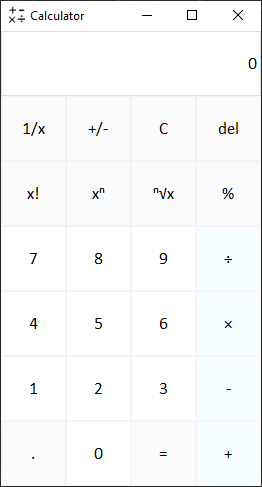
\includegraphics[scale=1]{calculator_GUI_screenshot.PNG}
  \caption{Calculator application}
  \label{fig:calculator}
\end{figure}

\subsection{Entering numbers}
Use the number panel for entering numbers.
If you need to delete the last character you wrote, press del (delete), or you can use the C button (clear) to clear all input to the calculator.\par

\subsection{Mathematical operations}
We distinguish two types of operations: unary (violet), which is an operation with a single operand, and binary (green), which needs two operands to successfully complete the operation.

\begin{figure}[H]
\centering
  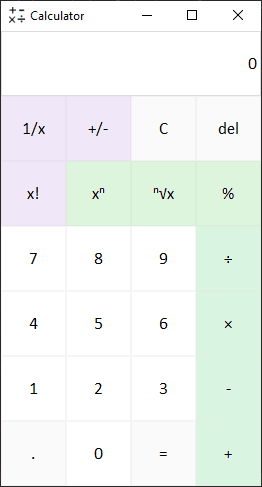
\includegraphics[scale=1]{unaryvsbinary.png}
  \caption{Distinguish between unary (violet) and binary (green) operations}
  \label{fig:operations}
\end{figure}

For unary operations, enter the number, then press the button of the unary operation you need to calculate. The result is displayed on the result label.

For binary operations, enter the number, then press the button of the binary operation you need to calculate. The first operand disappears, then you can enter the second number. The result is displayed on the result label after pressing equals button.
\newpage

\end{document}
